\documentclass{article}

\usepackage{fancyvrb}
\usepackage{graphicx}
\usepackage{float}

\begin{document}

\nocite{*}

\begin{center}
\Huge 
CS2001/CS2101 Week 5 Practical

\vspace{0.5cm}

\textbf{JUnit and TDD}

\vspace{1cm}
\LARGE
12th October 2020

\large
\vspace{1.5cm}

\textbf{Matriculation Number: 200002548}

\vspace{0.5cm}

\textbf{Tutor: Alex Konovalov}

\end{center}

\vspace*{3cm}

\tableofcontents

\newpage
\section{Introduction}
The aim of this practical was to follow the Test Driven Development (TDD) methodology, to create an implementation of an ADT interface in Java using the JUnit framework. The ADT interfaces in question were \verb+IVendingMachine+, \verb+IProductRecord+ and \verb+IVendingMachineProduct+. They outlined the operation of a basic vending machine, whereby different products were stored in discrete lanes, and products could be bought or sold from a specific lane. \\ \\ \noindent Test Driven Development is a type of software development whereby unit tests are written and ran before implementation. Therefore the implementation is forced to adhere to the test specification, producing a robust program. These unit tests should be focused and independent from each other, the environment they are ran in, and the order of execution. \\ \\ \noindent Therefore, unit tests and implementation of the interfaces were carried out sequentially, for all methods in each interface. The unit tests were to cover the full range of of cases. Defining what should happen in normal, edge and exceptional cases.
\noindent
\section{Design}
There were three different classes \verb+VendingMachineProduct+, \verb+ProductRecord+ and \verb+VendingMachine+ used to implement the respective \verb+IVendingMachineProduct+, \verb+IProductRecord+ and \verb+IVendingMachine+ interfaces. Overall implementation was designed to be as maintainable and efficient as possible. There were some considerations that had to be made to design where the specification was vague:
\begin{itemize}
	\item A lane is considered to be still open to a certain type of product even if there are no products left in the lane.
	\item Products with the same description can feature on multiple different lanes.
	\item There is no max limit on the number of items in each lane.
	\item \verb+IVendingMachineProduct+'s can have null \verb+laneCodes+ and \verb+desriptions+.
	\item A vending machine can initially have no products registered.
	\item If \verb+IVendingMachines+'s \verb+getMostPopular+ method comes across two \verb+IProdu+ \verb+ctRecords+ that have the same number of sales the most popular product is chosen to be the first product it encounters.
	
\end{itemize}
\subsection{VendingMachineProduct Class}
This class implements the \verb+IVendingMachineProduct+ interface. This class has a basic implementation, it stores two private string attributes, \verb+laneCode+ and \verb+description+ used to describe and identify a certain product that could feature in the \verb+VendingMachine+. It has two methods overridden from the interface that each return the laneCode or description. No restrictions were placed on the \verb+laneCode+ and \verb+description+ because it was not outlined as a requirement in the specification and would increase complexity without any real benefit.
\subsection{ProductRecord Class}
This class implements the \verb+IProductRecord+ interface. This class has three private attributes. The \verb+vendingMachineProduct+ variable of type \verb+IVendingMachine+ \verb+Product+ stores the product it is related to. Two integers are also used to keep track of the number of items available and the number sold. The \verb+buyItem()+ method increments the number of sales and decrements the number available by one. However if there are no products of that type available the method throws a \verb+ProductUnavailableException+. The \verb+addItem+ method does the opposite increments the number of items available by one.
\subsection{VendingMachine Class}
This class implements the \verb+IVendingMachine+ interface and has two private attributes. This first is a \verb+HashMap+ called \verb+products+. This is the collection used for storing the \verb+IProductRecord+'s stored by the \verb+VendingMachine+. The interface specified that a considerable number of methods would have as a parameter the string \verb+laneCode+. Therefore, it made sense to use a \verb+HashMap+ with \verb+laneCode+'s as keys as this would allow for easy access to a specific \verb+laneCode+ for these methods. This means that implementation was a lot easier than an array based implementation as \verb+contains()+ operations were faster, taking constant time - O(1). The second attribute is an integer to store the number of items within the entire \verb+VendingMachine+. This was added because it allows for constant time - O(1) - \verb+getTotalNumberOfItems()+ calls, since now the method can just return this number. Without it, the  method would have to iterate over every \verb+IProductRecord+ in the \verb+products+ \verb+HashMap+ to add up all the separate integers. \\ \\ \noindent The method \verb+registerProduct()+ checks to see if a product is in \verb+products+ before adding it. If the \verb+laneCode+ for the product is already in \verb+products+ then the function throws a \verb+LaneCodeAlreadyInUs+ \verb+eException+. \verb+unregisterProduct()+ checks if the laneCode is already in \verb+products+ and if it is removes the product from the machine. If not, it throws \verb+LaneCodeNotRegisteredException+. \\ \\ \noindent Both \verb+addItem()+ and \verb+removeItem()+ increment and decrement the number of a specific product by one, however if the \verb+laneCode+ specifying the product is not in \verb+products+ they throw a \verb+LaneCodeNotRegisteredException+. Furthermore, \verb+getNumberOfItems+ and \verb+getNumberOfsales+ return the sales and number of items available of a particular product. Again, if \verb+laneCode+ is not present in \verb+products+ the same exception is thrown. \\ \\ \noindent The \verb+getMostPopular()+ finds the \verb+IProductRecord+ in \verb+records+ with the most number of sales. If multiple products have the same number of sales the method picks the most popular product to be the first product it comes across. As per the interface, the method throws a \verb+LaneCodeNotRegisteredException+ if there are no products in \verb+products+.
\section{Testing}
There are in total 53 different tests associated with this project. However, if we remove parametrised tests this number falls to 41. Implementation has proven to be successful as all 53 tests passed, as shown in figure \ref{fig:test_results} and \ref{fig:test_results_console}. The tests were split into separate test classes with each test class testing each implementation of the interfaces. They were split up like this as it makes them easier to manage and diagnose which implementation is failing. In \verb+IVendingMachineProductTests+ there are 6 tests, \verb+IProductRecordTests+ has 11, and \verb+IVendingMachineTests+ includes 24.
\begin{figure}[h]
\centering
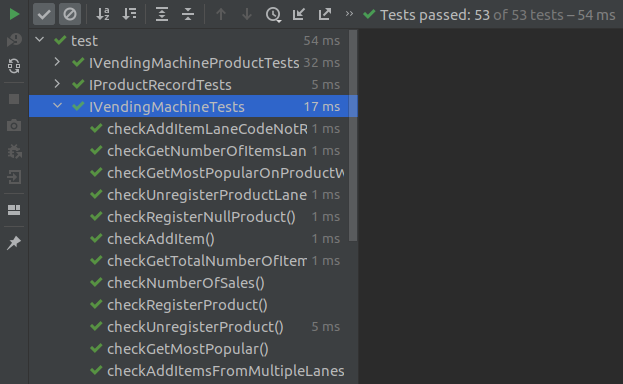
\includegraphics[width = 250px, clip]{test_results.png}
\caption{JUnit IntelliJ integration showing all tests passing}
\label{fig:test_results}
\end{figure}
\begin{figure}[h]
\centering
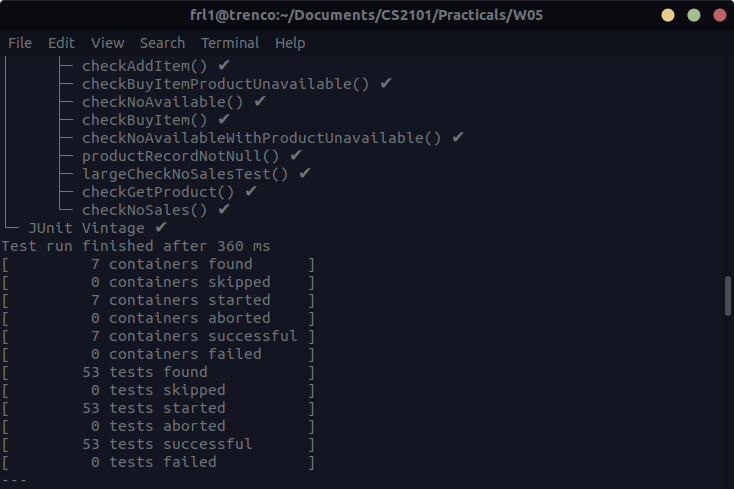
\includegraphics[width = 250px, clip]{test_results_console.png}
\caption{JUnit ran on stacscheck showing all tests passing}
\label{fig:test_results_console}
\end{figure}




\subsection{IVendingMachineProduct Tests}
\begin{itemize}
\item \verb+vendingMachineProductNotNull()+
\begin{itemize}
\item Tests that the factory was able to call a sensible constructor to get a non-null instance of IVendingMachineProduct.
\end{itemize}

\item \verb+checkDescriptionAndLaneCode()+
\begin{itemize}
\item Tests that the laneCode and description and are present in the instance of IVendingMachineProduct.
\item Included as we need to make sure that the laneCode and description are present in the object as otherwise this would cause other errors when trying to include them in the products HashMap in IVendingMachine.
\end{itemize}

\item \verb+checkDescription()+
\begin{itemize}
\item Tests that different descriptions (including single character and empty strings) are accepted by IVendingMachineProduct.
\item This is a parametrised test that takes in different product descriptions: \verb+"Haggis Crisps", "Chocolate", "", "a", " "+
\item Included as we need to make sure that when the method is implemented it can handle any string, whether it be empty, one character, one word or multiple words.
\end{itemize}

\item \verb+descriptionNull()+
\begin{itemize}
\item Tests that the IVendingMachineProduct description can be null.
\item Included as we need to ensure that we can handle null values in our description.
\end{itemize}

\item \verb+checkLaneCode()+
\begin{itemize}
\item Tests that different laneCodes (including single character and empty strings) are accepted by IVendingMachineProduct.
\item This is a parametrised test that takes in different lineCodes: \verb+"A1",+ \\ \verb+"A2", "A49320", "A0", "0A", "A0B", "394fj04", "", " "+
\item Included as there is no formal restrictions in the specification about the format of laneCodes and so should be able to be a string of any form. Here we consider if it is empty, one character, or multiple characters.
\end{itemize}

\item \verb+laneCodeNull()+
\begin{itemize}
\item Tests that the IVendingMachineProduct laneCode can be null.
\item Included as we need to ensure that we can handle null values as laneCodes.
\end{itemize}
\end{itemize}





\subsection{IProductRecord Tests}
This test class features a \verb+@BeforeEach+ method that runs creates a new \verb+IVending+ \verb+MachineProduct+ and \verb+IProductRecord+ before every test. This allows for each test to use standard variables that will be reset after every test, therefore removing dependency between tests.
\begin{itemize}

\item \verb+productRecordNotNull()+
\begin{itemize}
\item Tests that the factory was able to call a sensible constructor to get a non-null instance of IProductRecord.
\end{itemize}

\item \verb+checkGetProduct()+
\begin{itemize}
\item Tests that the IProductRecord can still retrieve the correct IVendingMachineProduct using the getProduct() method and that the IVendingMachineProduct holds the correct laneCode and description.
\item Included since receiving the IVendingMachineProduct needs to be correct since so that methods can work correctly later on within the IVendingMachine implementation.
\end{itemize}

\item \verb+checkBuyItem()+
\begin{itemize}
\item Tests that the buyItem() method works in buying an item that is available.
\item Included since we need to make sure that an item can be bought for future tests and within the IVendingMachine implementation.
\end{itemize}

\item \verb+checkAddItem()+
\begin{itemize}
\item Tests that the addItem() method works to add one new item to IProductRecord.
\item Included since we need an item to be added to the IVendingMachine so that it can be later bought.
\end{itemize}

\item \verb+checkBuyItemProductUnavailable()+
\begin{itemize}
\item Tests that the buyItem() method throws a ProductUnavailableException when buying an item that not available. It checks this before any items have been added, and after an item has been bought and is no longer available.
\item Included since buying an item when it is not available should throw this exception up to the IVendingMachine to let the user know that there are no items left and that more need to be added.
\end{itemize}

\item \verb+checkNoAvailable()+
\begin{itemize}
\item Tests that the getNumberAvailable() method correctly returns the number of products available after multiple buyItem() and addItem() method calls.
\item Included since we need to make sure that the IProductRecord implementation counts the number of items added and bought correctly.
\end{itemize}

\item \verb+checkNoSales()+
\begin{itemize}
\item Tests that the getNumberOfSales() method correctly returns the number of products sold after multiple items have been bought.
\item Included since we need to make sure that the IProductRecord implementation counts the number of items bought correctly.
\end{itemize}

\item \verb+checkNoSalesWithProductUnavailable()+
\begin{itemize}
\item Tests that the number of sales does not change after the buyItem() method throws a ProductUnavailableException if a product has tried to be sold that is not available.
\item Included since we need to make sure that the number of sales does not change if we receive a ProductUnavailableException since if this error has been generated a product should not be able to be bought.
\end{itemize}

\item \verb+checkNoAvailableWithProductUnavailable()+
\begin{itemize}
\item Tests that the amount of product available does not change after the buyItem() method throws a ProductUnavailableException if a product has tried to be sold that is not available.
\item Included since we need to make sure that the number of products available does not change if we receive a ProductUnavailableException. If we do not check this then the number available could be going into negative numbers since no available could be decremented when nothing has been sold.
\end{itemize}

\item \verb+largeCheckNoAvailableTest()+
\begin{itemize}
\item Tests that IProductRecord can add lots of the same item and can return the correct number of items available.
\item Included since there should be no limit (or to a high a limit to notice there is one) on the number of products that can be available in the IVendingMachine. This was specified in the design.
\end{itemize}

\item \verb+largeCheckNoSalesTest()+
\begin{itemize}
\item Tests that IProductRecord can buy lots of the same item and can return the correct number of products sold.
\item Included since there should be no limit (or to a high a limit to notice there is one) on the number of products that can be sold in the IVendingMachine. This was specified in the design.
\end{itemize}
\end{itemize}




\subsection{IVendingMachine Tests}
This test class also features a \verb+@BeforeEach+ method that runs creates a new \verb+IVendingMachine+ and two \verb+IProductRecord+'s before every test. This allows for each test to use standard variables that will be reset after every test, therefore removing dependency between tests.

\begin{itemize}

\item \verb+vendingMachineNotNull()+
\begin{itemize}
\item Tests that the factory was able to call a sensible constructor to get a non-null instance of IVendingMachine.
\end{itemize}

\item \verb+checkRegisterProduct()+
\begin{itemize}
\item Tests that a product has been successfully registered within the IVendingMachine in a specific lane.
\item Included since products should be able to be registered to the IVendingMachine if a IProductRecord object is passed in.
\end{itemize}

\item \verb+checkRegisterNullProduct()+
\begin{itemize}
\item Tests that IVendingMachine throws a NullPointerException when trying to register a null product.
\item Included since if a null value is trying to be registered as a product this should throw an error.
\end{itemize}

\item \verb+checkRegisterProductLaneAlreadyInUse()+
\begin{itemize}
\item Tests that the IVendingMachine throws a LaneCodeAlreadyInUseException when trying to register a product that has already been registered to that lane code in the machine.
\item Included since if a product lane is already in use and another product is trying to be registered in that product lane this should cause a LaneCodeAlreadyInUseException and not register two products in one lane.
\end{itemize}

\item \verb+checkUnregisterProduct()+
\begin{itemize}
\item Tests that a product has been successfully unregistered from the IVendingMachine and is no longer available.
\item Included since we need to check if a product has been unregistered so that we can register products back to the lane later.
\end{itemize}

\item \verb+checkUnregisterProductLaneCodeNotRegistered()+
\begin{itemize}
\item Tests that the IVendingMachine throws a LaneCodeNotRegisteredException when trying to unregister a product that does not exist.
\item Included since we should not be able to unregister a product if it does not exit in the IVendingMachine.
\end{itemize}

\item \verb+checkAddItem()+
\begin{itemize}
\item Tests that a IVendingMachine adds an item on the specified lane.
\item Included since we need to know if items are being added onto the specified lane correctly.
\end{itemize}

\item \verb+checkAddItemsFromMultipleLanes()+
\begin{itemize}
\item Tests that IVendingMachine adds two different products on separate lanes correctly.
\item Included since we need to know if items are being added onto the specified lanes correctly when dealing with adding to multiple different lanes at the same time.
\end{itemize}

\item \verb+checkAddItemLaneCodeNotRegistered()+
\begin{itemize}
\item Tests that the IVendingMachine throws a LaneCodeNotRegisteredException when trying to add an item to a lane code that does not exist.
\item Included since it should not be possible to add an item to a lane code and IProductRecord that does not exist.
\end{itemize}

\item \verb+checkBuyItem()+
\begin{itemize}
\item Tests that a IVendingMachine buys an item from the specified lane.
\item Included since we need to know if items are being bought onto the specified lane correctly.
\end{itemize}

\item \verb+checkBuyItemLaneCodeNotRegistered()+
\begin{itemize}
\item Tests that the IVendingMachine throws a LaneCodeNotRegisteredException when trying to buy an item from a lane code that does not exist.
\item Included since it should not be possible to buy an item from a lane code and IProductRecord that does not exist.
\end{itemize}

\item \verb+checkBuyItemsFromMultipleLanes()+
\begin{itemize}
\item Tests that IVendingMachine buys two different products from separate lanes correctly.
\item Included since we need to know if items are being bought from the specified lanes correctly when dealing with adding to multiple different lanes at the same time.
\end{itemize}

\item \verb+checkBuyItemsProductUnavailable()+
\begin{itemize}
\item Tests that IVendingMachine throws a ProductUnavailableException when trying to buy an item from a lane in which there are no products left to buy.
\item Included since if there are no products left to buy then the ProductUnavailableException should be thrown and no items of the product should be bought since the amount of products available cannot be a negative number.
\end{itemize}

\item \verb+checkGetNumberOfProducts()+
\begin{itemize}
\item Tests that the correct value for the number of products registered is returned by the IVendingMachine class.
\end{itemize}

\item \verb+checkGetTotalNumberOfItems()+
\begin{itemize}
\item Tests that IVendingMachine calculates the correct value for the total number of items over all products in the machine. The test checks if this value is correct when we add and buy multiple items from multiple lanes in the IVendingMachine.
\item Included since we need to check that the system for incrementing the noOfItems variable works correctly. This is needed since we included this variable rather than iterate over all of the products.
\end{itemize}

\item \verb+checkGetNumberOfItems()+
\begin{itemize}
\item Tests that IVendingMachine returns the correct value for the total number of items of one product. The test checks if this value is correct when we add and buy multiple items from multiple lanes (which should not update the value if not in the chosen lane) in the IVendingMachine. 
\end{itemize}

\item \verb+checkGetNumberOfItemsLaneCodeNotRegistered()+
\begin{itemize}
\item Tests that IVendingMachine throws a LaneCodeNotRegisteredException when trying to check for the number of items of a product in a lane code that does not exist.
\item Included since a LaneCodeNotRegisteredException should occur because the number of items in an unregistered lane is undefined.
\end{itemize}

\item \verb+checkNumberOfSales()+
\begin{itemize}
\item Tests that IVendingMachine returns the correct value for the total number of sales of one product. The test checks if this value is correct when buying multiple items from multiple lanes (which should not update the value if not in the chosen lane) in the IVendingMachine.
\end{itemize}

\item \verb+checkGetNumberOfSalesLaneCodeNotRegistered()+
\begin{itemize}
\item Tests that IVendingMachine throws a LaneCodeNotRegisteredException when trying to check for the number of sales of a product in a lane code that does not exist.
\item Included since a LaneCodeNotRegisteredException should occur because the number of sales in an unregistered lane is undefined.
\end{itemize}

\item \verb+checkGetMostPopular()+
\begin{itemize}
\item Tests that the most popular product is calculated to be the product bought the most number of times.
\item Included since we need an initial test to see that the getMostPopular method works in a normal test case where there is a clear most popular product out of multiple products.
\end{itemize}

\item \verb+checkGetMostPopularLaneCodeNotRegistered()+
\begin{itemize}
\item Tests that IVendingMachine throws a LaneCodeNotRegisteredException when trying to check for the most popular product when no products have registered yet.
\item Included since if no products have been registered yet then a LaneCodeNotRegisteredException should be thrown because there is no IProductRecord to return.
\end{itemize}

\item \verb+checkGetMostPopularOnProductWithNoItems()+
\begin{itemize}
\item Tests that IVendingMachine can return the most popular product when products with no items are present in the machine.
\item Included since we need to text extreme cases where the most popular product is default the only one in the IVendingMachine, even though it has no sales.
\end{itemize}

\item \verb+checkGetMostPopularOnProductWithOneProduct()+
\begin{itemize}
\item Tests that IVendingMachine can return the most popular product when only one product is present but has items in the machine.
\item Included since this extreme test should return the most popular product to be the only product that has sold.
\end{itemize}

\item \verb+checkGetMostPopularWithTiedProducts()+
\begin{itemize}
\item Tests that IVendingMachine can return the most popular product when multiple products have the same number of sales. This should return the first product it comes across as the behaviour is undefined.
\item Included since this extreme test should return the first product it comes across that is one of the most popular products and not anything else.
\end{itemize}

\end{itemize}
\section{Conclusion}
In this practical I followed TDD methodology whilst using the JUnit framework to implement the three ADT interfaces, \verb+IVendingMachine+, \verb+IProductRecord+ and \verb+IVendingMachineProduct+. I wrote test methods to first establish the behaviour of methods I was implementing, and ran these implementations through the test methods I defined. These tests cover the full range of test cases, from normal to extreme and exceptional test cases. I learnt a lot about the TDD process, JUnit and factories. Using IntelliJ with JUnit was excellent as it had inbuilt testing features, making it easy find out where and why some tests failed without leaving the IDE. \\ \\ \noindent Overall, implementation in this project was not too challenging. The difficult aspect of the practical was in designing tests that covered all normal, extreme and exceptional test cases. I enjoyed using JUnit and found that different assertions and \verb+@BeforeEach+ made it extremely easy to test my various implementations. While I can now appreciate the benefits of TDD, I would still be unlikely to use it over the traditional software development process. I feel like it is suited to a smaller, subset of programming projects, where there can only be a small number of outcomes. That said, if I was building a small implementation of an ADT again, that I needed to ensure was as robust as possilbe, TDD would be a good approach to utilise.
\begin{thebibliography}{10}
\bibitem{numeric}
Stefan Bechtold, Sam Brannen, Johannes Link, Matthias Merdes, Marc Philipp, Juliette de Rancourt, Christian Stein, \textit{JUnit 5 User Guide V5.7.0}, 14-08-2020, accessed 13-10-2020, \\\texttt{https://junit.org/junit5/docs/current/user-guide/}

\bibitem{numeric}
JetBrains, \textit{Prepare for testing}, 19-08-2020, accessed 13-10-2020, \\\texttt{https://www.jetbrains.com/help/idea/testing.html}

\end{thebibliography}
\end{document}